\chapterimage{chapter-t2-bg} % Chapter heading image

\chapter{Interface Guide}

The way stellarium is shown on the screen is primarily governed by the
menus. These are accessed by dragging the mouse to the left or bottom
edge of the screen

\section{Tour}\index{Tour}

\begin{figure}[h]
\centering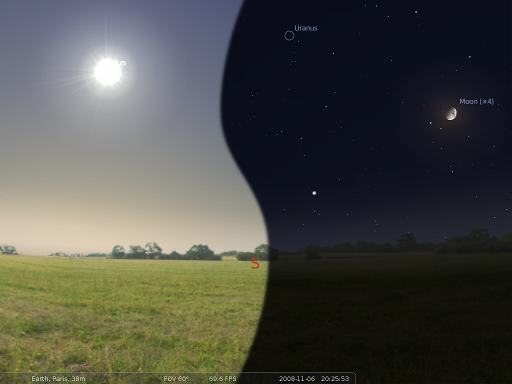
\includegraphics{001}
%\caption{Figure caption}
\end{figure}

At the bottom left of the screen, you can see the status bar. This shows
the current observer location, field of view (FOV), graphics performance
in frames per second (FPS) and the current simulation date and time.

The rest of the view is devoted to rendering a realistic scene including
a panoramic langscape and the sky. If the simulation time and observer
location are such that it is night time, you will see stars, planets and
the moon in the sky, all in the correct positions.

You can drag with the mouse on the sky to look around or use the cursor
keys. You can zoom with the mouse wheel or the page up/page down keys.

If you move the mouse over the status bar, it will move up to reveal a
tool bar which gives quick control over the program.

\subsection{Time Travel}\index{Time Travel}

When Stellarium starts up, it sets its clock to the same time and date
as the system clock. However, Stellarium's clock is not fixed to same
time and date as the system clock, or indeed to the same speed. We may
tell Stellarium to change how fast time should pass, and even make time
go backwards! So the first thing we shall do is to travel into the
future! Let's take a look at the time control buttons on the right hand
ride of the tool-bar. If you hover the mouse cursor over the buttons, a
short description of the button's purpose and keyboard shortcut will
appear.

\begin{table}[h]
\centering
\begin{tabular}{c c l}
\toprule
\textbf{Button} & \textbf{Shortcut key} & \textbf{Description}\\
\midrule

\includegraphics[scale=0.75]{timerate_decrease} & J & Decrease the rate at which time passes \\

\includegraphics[scale=0.75]{timerate_normal} & K & Make time pass as normal \\

\includegraphics[scale=0.75]{timerate_increase} & L & Increase the rate at which time passes \\

\includegraphics[scale=0.75]{time_normal} & 8 & Return to the current time \& date \\
\bottomrule
\end{tabular}
\caption{Time Travel}
\end{table}

OK, so lets go see the future! Click the mouse once on the increase time
speed button

\includegraphics[scale=0.5]{timerate_increase}
. Not a whole lot seems to happen. However, take a look at the clock in
the status bar. You should see the time going by faster than a normal
clock! Click the button a second time. Now the time is going by faster
than before. If it's night time, you might also notice that the stars
have started to move slightly across the sky. If it's daytime you might
be able to see the sun moving (but it's less apparent than the movement
of the stars). Increase the rate at which time passes again by clicking
on the button a third time. Now time is really flying!

Let time move on at this fast speed for a little while. Notice how the
stars move across the sky. If you wait a little while, you'll see the
Sun rising and setting. It's a bit like a time-lapse movie. Stellarium
not only allows for moving forward through time - you can go backwards
too!

Click on the real time speed button

\includegraphics[scale=0.5]{timerate_normal} .
The stars and/or the Sun should stop scooting across the sky. Now press
the decrease time speed button

\includegraphics[scale=0.5]{timerate_decrease}
once. Look at the clock. Time has stopped. Click the Decrease time speed
button four or five more times. Now we're falling back through time at
quite a rate (about one day every ten seconds!).

Enough time travel for now. Wait until it's night time, and then click
the Real time speed button. With a little luck you will now be looking
at the night sky.

\subsection{Moving Around the Sky}\index{Moving Around the Sky}

\begin{table}[h]
\centering
\begin{tabular}{l l}
\toprule
\textbf{Key} & \textbf{Description}\\
\midrule
Cursor keys & Pan the view left, right, up and down \\
Page up / Page down & Zoom in and out \\
Backslash (\textbackslash{}) & Auto-zoom out to original field of
view \\
Left mouse button & Select an object in the sky \\
Right mouse button & Clear selected object \\
Mouse wheel & Zoom in and out \\ 
Space & Centre view on selected object \\
Forward-slash (/) & Auto-zoom in to selected object \\
\bottomrule
\end{tabular}
\caption{Moving Around the Sky}
\end{table}

As well as travelling through time, Stellarium lets to look around the
sky freely, and zoom in and out. There are several ways to accomplish
this listed in table above.

Let's try it. Use the cursors to move around left, right, up and down.
Zoom in a little using the Page Up key, and back out again using the
Page Down. Press the backslash key and see how Stellarium returns to the
original field of view (how ``zoomed in'' the view is), and direction of
view.

It's also possible to move around using the mouse. If you left-click and
drag somewhere on the sky, you can pull the view around.

Another method of moving is to select some object in the sky (left-click
on the object), and press the Space key to centre the view on that
object. Similarly, selecting an object and pressing the forward-slash
key will centre on the object and zoom right in on it.

The forward-slash and backslash keys auto-zoom in an out to different
levels depending on what is selected. If the object selected is a planet
or moon in a \emph{sub-system} with a lot of moons (e.g. Jupiter), the
initial zoom in will go to an intermediate level where the whole
sub-system should be visible. A second zoom will go to the full zoom
level on the selected object. Similarly, if you are fully zoomed in on a
moon of Jupiter, the first auto-zoom out will go to the sub-system zoom
level. Subsequent auto-zoom out will fully zoom out and return the
initial direction of view. For objects that are not part of a
sub-system, the initial auto-zoom in will zoom right in on the selected
object (the exact field of view depending on the size/type of the
selected object), and the initial auto-zoom out will return to the
initial FOV and direction of view.

\subsection{Main Tool-bar}\index{Main Tool-bar}

\begin{figure}[h]
\centering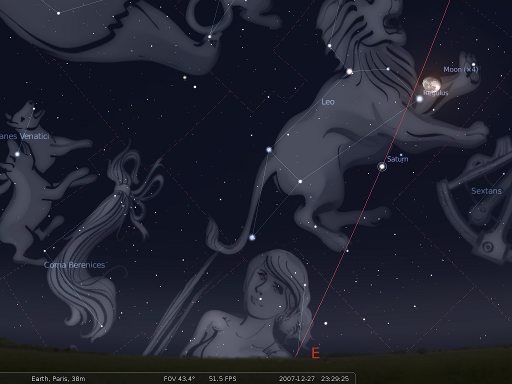
\includegraphics{002}
%\caption{Figure caption}
\end{figure}

Stellarium can do a whole lot more than just draw the stars. Figure
above shows some of Stellarium's visual effects including constellation
line and boundary drawing, constellation art, planet hints, and
atmospheric fogging around the bright Moon. The controls main tool-bar
provides a mechanism for turning on and off the visual effects.

When the mouse if moved to the bottom left of the screen, a second
tool-bar becomes visible. All the buttons in this side tool-bar open and
close dialog boxes which contain controls for further configuration of
the program.

Table below describes the operations of buttons on the main tool-bar and
the side tool-bar, and gives their keyboard shortcuts.

\begin{longtabu} to \textwidth {l l l X}
\toprule
\textbf{Feature} & \textbf{Button} & \textbf{Key} & \textbf{Description}\\
\midrule
Constellations & 
\includegraphics[scale=0.75]{constellation_button} & C & Draws the constellation lines \\
Constellation Names & 
\includegraphics[scale=0.75]{constellation_name_button}
& V & Draws the name of the constellations \\
Constellation Art & 
\includegraphics[scale=0.75]{constellation_art_button}
& R & Superimposes artistic representations of the constellations over
the stars \\
Equatorial Grid & 
\includegraphics[scale=0.75]{eq_grid_button} & E &
Draws grid lines for the RA/Dec coordinate system \\
Azimuth Grid & 
\includegraphics[scale=0.75]{az_grid_button} & Z &
Draws grid lines for the Alt/Azi coordinate system \\
Toggle Ground & 
\includegraphics[scale=0.75]{ground_button} & G &
Toggles drawing of the ground. Turn this off to see objects that are
below the horizon \\
Toggle Cardinal Points & 
\includegraphics[scale=0.75]{cardinal_button} & Q &
Toggles marking of the North, South, East and West points on the
horizon \\
Toggle Atmosphere & 
\includegraphics[scale=0.75]{atmosphere_button} & A
& Toggles atmospheric effects. Most notably makes the stars visible in
the daytime \\
Deep-Sky Objects & 
\includegraphics[scale=0.75]{nebulae_button} & D &
Toggles marking the positions of Deep-Sky Objects when the FOV is
too wide to see them \\
Planet Hints & 
\includegraphics[scale=0.75]{planets_button} & P &
Toggles indicators to show the position of planets \\
Coordinate System & 
\includegraphics[scale=0.75]{coord_type_button} &
Enter & Toggles between Alt/Azi \& RA/Dec coordinate systems \\
Goto & 
\includegraphics[scale=0.75]{goto_button} &
Space & Centres the view on the selected object \\
Night Mode & 
\includegraphics[scale=0.75]{night_mode_button} &
Ctrl+N & Toggle ``night mode'', which changes the coloring of same
display elements to be easier on the dark-adapted eye. \\
Nebula background images & 
\includegraphics[scale=0.75]{DSS_button} &
{[}none{]} & Toggle ``nebula background images'', which turns the
Textures on or off. \\
Full Screen Mode & 
\includegraphics[scale=0.75]{fullscreen_button} &
F11 & Toggle full screen mode. \\
Flip image (horizontal) & 
\includegraphics[scale=0.75]{fliph_button} &
Ctrl+Shift+H & Flips the image in the horizontal plane. Note this button
is not enable by default. See section {[}sec:imageflipping{]} \\
Flip image (vertical) & 
\includegraphics[scale=0.75]{flipv_button} &
Ctrl+Shift+V & Flips the image in the vertical plane. Note this button
is not enable by default. See section {[}sec:imageflipping{]} \\
Quit Stellarium & 
\includegraphics[scale=0.75]{quit_button} & Ctrl-Q
& Close Stellarium. Note: the keyboard shortcut is COMMAND-Q on OSX
machines \\
Help Window & 
\includegraphics[scale=0.5]{help_button} & F1 &
Show the help window, which lists key bindings and other useful
information \\
Configuration Window & 
\includegraphics[scale=0.5]{config_button} & F2 &
Show the display of the configuration window \\
Search Window & 
\includegraphics[scale=0.5]{find_button} & F3 or
Ctrl+F & Show the display of the object search window \\
View Window & 
\includegraphics[scale=0.5]{view_button} & F4 &
Show the view window \\
Time Window & 
\includegraphics[scale=0.5]{time_button} & F5 &
Show the display of the help window \\
Location Window & 
\includegraphics[scale=0.5]{location_button} & F6
& Show the observer location window (map) \\
\bottomrule
\end{longtabu}

\subsection{The Object Search Window}\index{The Object Search Window}

\begin{figure}[h]
\centering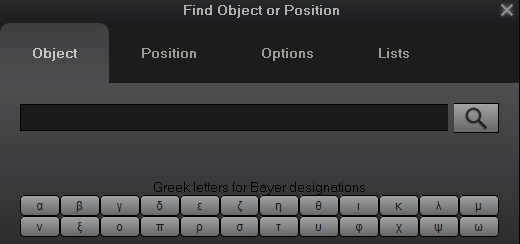
\includegraphics{search_dialog}
\caption{The Object Search Window}
\end{figure}

The Object Search window provides a convenient way to locate objects in
the sky. Simply type in the name of an object to find, and then click
the ``go'' button or press return. Stellarium will point you at that
object in the sky.

As you type, Stellarium will make a list of objects which begin with
what you have typed so far. The first of the list of matching objects
will be highlighted. If you press the TAB key, the selection will change
to the next item in the list. Hitting the RETURN key will go to the
currently highlighted object and close the search dialog.

For example, suppose we want to locate Mimas (a moon of Saturn). After
typing the first letter of the name, \emph{m}, Stellarium makes a list
of objects whose name begins with M: Mars, Mercury, Mimas, Miranda,
Moon. The first item in this list, Mars, is highlighted. Pressing return
now would go to Mars, but we want Mimas. We can either press TAB twice
to highlight Mimas and then hit RETURN, or we can continue to type the
name until it is the first/only object in the list.

\begin{figure}[h]
\centering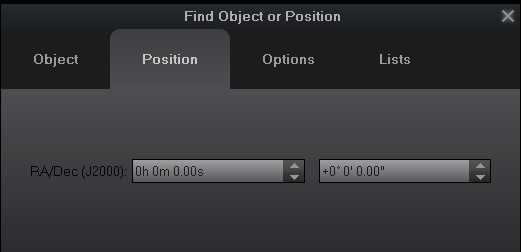
\includegraphics{search_dialog_position}
%\caption{The Object Search Window}
\end{figure}

The Position Search window provides a convenient way to enter a user set
of coordinateslocate objects in the sky. Simply type in the name of an
object to find, and then click the ``go'' button or press return.
Stellarium will point you at that object in the sky.

\begin{figure}[h]
\centering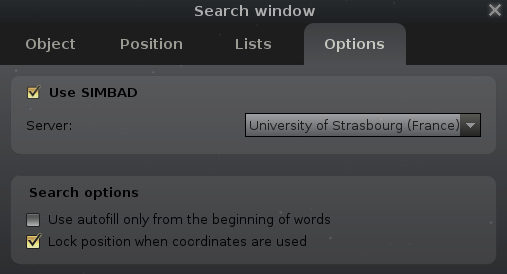
\includegraphics{search_dialog_option}
%\caption{The Object Search Window}
\end{figure}

The Option Search window provides a convenient way to locate objects in
the sky. When the name of an object to find is typed in the object
window and you are connected to the internet and the Extended search is
ticked Stellarium will search the on line SIMBAD data bases for its
coordinates you can and then click the ``go'' button or press return.
Stellarium will point you at that object in the sky even if there is no
object displayed on the screen. The SIMBAD server being used can be
selected from the scroll window

\begin{figure}[h]
\centering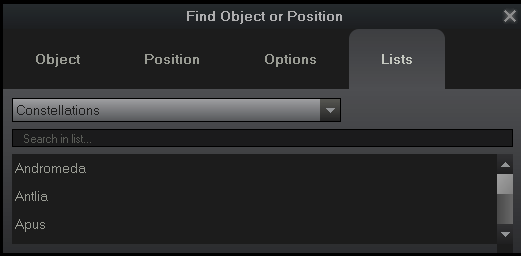
\includegraphics{search_dialog_list}
%\caption{The Object Search Window}
\end{figure}

The List Search window provides a convenient way to locate particular
types of objects in the sky. At the moment the number of choices is
governed by the loaded plug ins. Simply scroll down the first window to
select the type. The name of an object can then be selected from the
list. Press enter and stelarium will go to that object.

\subsection{Help Window}\index{Help Window}

\begin{figure}[h]
\centering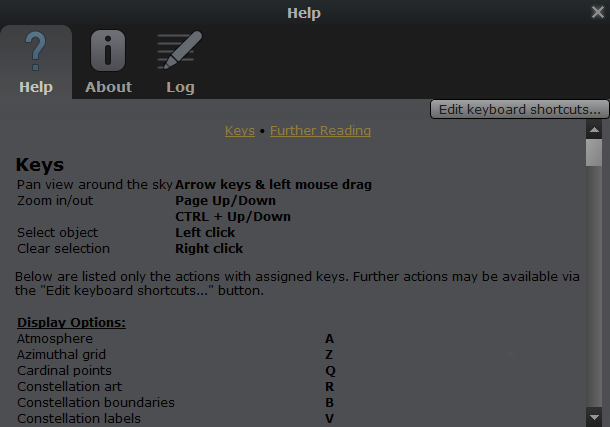
\includegraphics{help_dialog}
\caption{Help Window}
\end{figure}

The Help window lists all Stellarium's key-strokes. Not that some
features are only available as key strokes, so it's a good idea to have
a browse of the information in this window.

\begin{figure}[h]
\centering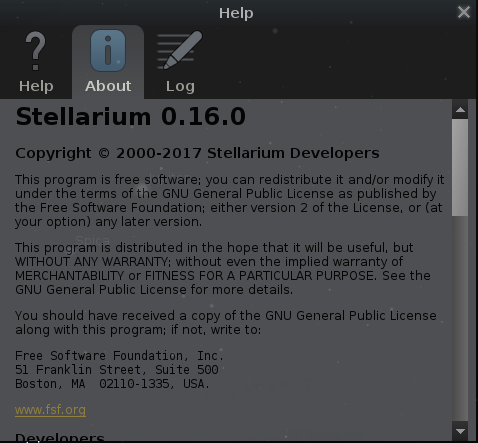
\includegraphics{help_dialog_about}
%\caption{Help Window}
\end{figure}

The About tab in this window will show licensing information, and a list
of people who helped to produce the program.

\begin{figure}[h]
\centering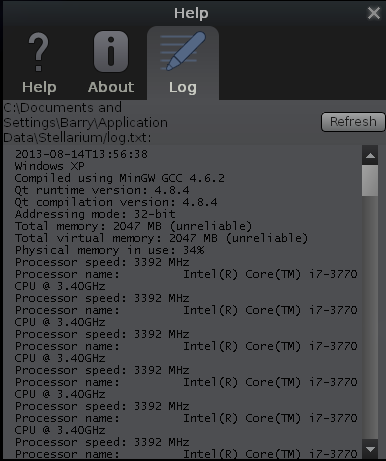
\includegraphics{help_dialog_log}
%\caption{Help Window}
\end{figure}

The help window log lists the loading instructions carried out when
stellarium runs. It is useful to locate the files that stellarium writes
to you computer. It is the master of the copy ``log.txt'' that you will
find in your user area.
